\documentclass[titlepage]{article}
\usepackage{amsthm,amssymb,amsmath,latexsym,graphicx, epsf, float, gensymb}
\usepackage[serbian]{babel}	
\usepackage[T1]{fontenc}
%\newcommand{\qed}{\hfill $\Box$\vspace*{4mm}}
\newtheorem{thm}{Teorema}[section]

\theoremstyle{remark}
\newtheorem{rem}[thm]{Napomena}

\theoremstyle{definition}
\newtheorem{df}[thm]{Definicija}

\newtheoremstyle{algorithm}	
{\topsep}                    % Space above
    {\topsep}                    % Space below
    {\itshape}                   % Body font
    {}                           % Indent amount
    {\scshape}                   % Theorem head font
    {:}                          % Punctuation after theorem head
    {\newline}                       % Space after theorem head
    {}  % Theorem head spec (can be left empty, meaning �normal�)

\theoremstyle{algorithm}
\newtheorem*{alg}{Algoritam}

\begin{document}

	\title{\sc Program za re\v{s}avanje Rubikove Kocke}
	\maketitle

    \section{Notacija}
        \textbf{Strane kocke} su obele\v{z}ene slovima $F, B, U, D, L, R$, i pri tome je:
        \begin{description}
          \item[F] prednja strana kocke
          \item[B] zadnja strana kocke
          \item[U] vrh kocke
          \item[D] dno kocke
          \item[L] leva strana kocke
          \item[R] desna strana kocke
        \end{description}
        \begin{figure}[H]
            \centering
            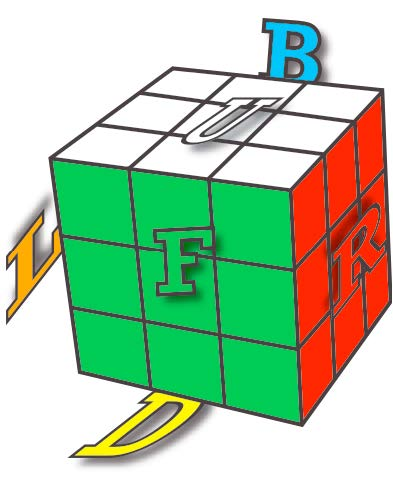
\includegraphics[scale=1]{images/faces.jpg}
            \caption{Strane kocke}
        \end{figure}
        Potezi su tako\dj e obele\v{z}eni slovima $F, B, U, D, L, R$, kao i stringovima $IF, IB, IU, ID, IL, IR$, gde su:
        \begin{description}
          \item[F i IF] okreti prednje strane za $-90\degree$ odnosno $90\degree$
          \item[B i IB] okreti zadnje strane za $-90\degree$ odnosno $90\degree$
          \item[U i IU] okreti vrha za $-90\degree$ odnosno $90\degree$
          \item[D i ID] okreti dna za $-90\degree$ odnosno $90\degree$
          \item[L i IL] okreti leve strane za $-90\degree$ odnosno $90\degree$
          \item[R i IR] okreti desne strane za $-90\degree$ odnosno $90\degree$
        \end{description}
        \begin{figure}[H]
            \centering
            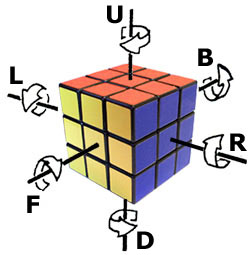
\includegraphics[scale=0.8]{images/notation.jpg}
            \caption{Potezi}
        \end{figure}
\end{document} 